\subsection{Measurement Noise}
\label{subsec:res-noise}
Fig.~\ref{fig:spectrum} shows the spectrum of a 100-ms record of D2: the four tones stand out over a flat floor, and the flicker of the room lights is confined to low frequencies. The noise of the RSS~\eqref{eq:lockin} was estimated from the same projection at off-tone frequencies, 20 to 40~kHz away from each tone, in the 1\,250 records of D2. Its standard deviation is $\sigma=1.92~\mu$V at 500~kHz; its 95th percentile over the records, which span all orientations and positions, is only 7\,\% higher (2.06~$\mu$V), which justifies a common value for all orientations, and 1.9--2.1~$\mu$V at the other tones. Over D2, the 500~kHz RSS ranges from 1.07 to 20.7~mV, so the SNR $s_i/\sigma$ lies between 573 and 10\,190 (median 4\,540). Consecutive records at the same pose, available for 47 poses, differ by a median relative standard deviation of 0.019\,\% (P90 0.037\,\%), as expected from this floor alone; within a record time, neither the LED nor the receiver chain adds noticeable fluctuations. Measurement noise is therefore small, and the question is whether it limits the accuracy (Section~\ref{subsec:res-bound}).

\begin{figure}[!t]
 \centering
 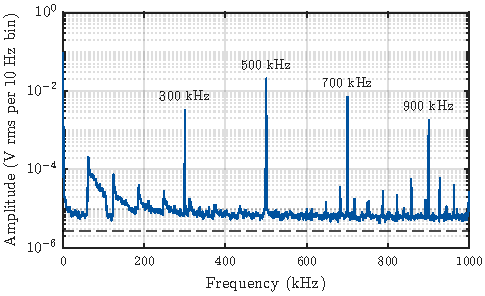
\includegraphics[width=\linewidth]{fig_spectrum.pdf}
 \caption{Amplitude spectrum of a 100-ms record of D2 (maximum over 1-kHz groups of 10-Hz bins). The four LED tones are separated in frequency; the dashed line is the median off-tone floor at 500~kHz.}
 \label{fig:spectrum}
\end{figure}

\subsection{LED Radiation Patterns}
\label{subsec:res-env}
Fig.~\ref{fig:maps} shows the flat-PD maps of D1 for the four LEDs. Each LED has a single smooth lobe, without visible reflections, and the joint fit of~\eqref{eq:led-calibration} locates the center of its pattern ($+$). For the 500~kHz LED this center is at $(281.1,904.8)$~mm, the value of Table~\ref{tab:parameters}.

The pattern does not follow a single cosine power, however. Fig.~\ref{fig:calibration}(a) shows the apparent order of each point of D1, computed with $A$ fixed by the point closest to the axis. It decreases from about 11 near the axis to a stable value of 6.0 beyond $\phi\approx20^\circ$. The measured product $R(\phi)\cos^m\phi$ is thus more peaked near the axis than the model; the data constrain only this product, so the deviation may originate in the LED optics, in the response of the PD near normal incidence, or in a slight tilt of the LED. The staged calibration gives $m=6.09$, close to the value beyond $20^\circ$, where most positions of the working area are seen; a joint fit over the whole map gives $A=0.0611$~V\,m$^2$ and $m=5.79$.

\begin{figure*}[!t]
 \centering
 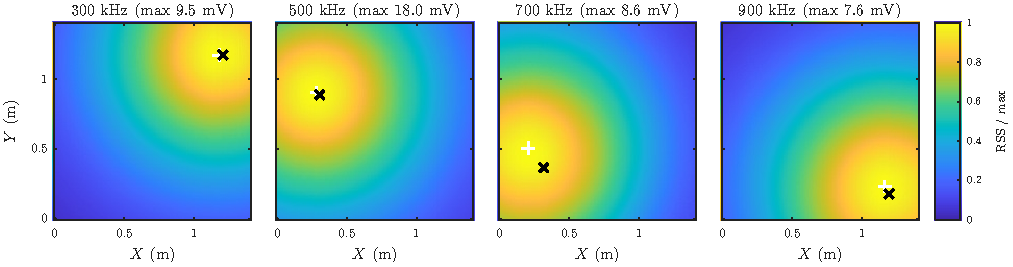
\includegraphics[width=\textwidth]{fig_maps.pdf}
 \caption{Flat-PD RSS maps of D1 (PD height 1.135~m, 10~mm grid), normalized by their maxima. $+$: center of the radiation pattern, from the joint fit of~\eqref{eq:led-calibration}; $\times$: geometric position of the LED, triangulated from its own estimated directions at the known positions of D2 (Section~\ref{subsec:res-leds}).}
 \label{fig:maps}
\end{figure*}

\subsection{Receiver Response Model}
\label{subsec:res-model}
Table~\ref{tab:models} compares the three response families on D2. The shape test~\eqref{eq:shape} at the true positions does not involve $A$, $m$ or the LED pattern; it gives a residual of 0.80\,\% for SQ, 1.42\,\% for $\cos^{1.9}$ and 6.63\,\% for $\cos$, with the stage zero fitted for each model (with the nominal $65^\circ$: 0.88, 1.47 and 6.63\,\%). The positioning results follow the same order. The Lambertian receiver $\cos\psi$ underestimates the decay of the response with the incidence angle; to explain the measured contrast between orientations it places the LED at a much larger zenith angle (direction errors of $11^\circ$--$12^\circ$), and the range stage converts this into errors of 0.7--0.8~m, with 10 and 9 failures for GLS and WLS. The cosine order fitted to the same device~\cite{Bastiaens2020} reduces the error to 8.2~cm, still more than twice that of SQ, with a vertical bias of $-5.6$~cm. A model that fits amplitudes reasonably well can still misrepresent their slopes (Section~\ref{subsec:fim}), and the shape test exposes it.

With the SQ response, GLS and NLS agree within 0.01~cm, as expected at high SNR; WLS ignores the correlation between ratios that share a reference and is slightly worse. NLS is used in the following.

\begin{table}[!t]
 \centering
 \caption{Receiver Models and Estimators on D2 (125 Positions, $K=10$)}
 \label{tab:models}
 \footnotesize
 \setlength{\tabcolsep}{3.2pt}
 \begin{tabular}{@{}llccccc@{}}
 \toprule
 Response & Estim. & $\rho$ (\%) & Mean & P90 & Vert. & Fail.\\
 & & & (cm) & (cm) & (cm) & \\
 \midrule
 $\cos\psi$ & GLS & 6.63 & 71.8 & 131.0 & $+67.6$ & 10\\
 & WLS & & 76.1 & 131.9 & $+71.9$ & 9\\
 & NLS & & 76.8 & 134.5 & $+72.1$ & 0\\
 $\cos^{1.9}\psi$ & GLS & 1.42 & 8.21 & 12.80 & $-5.55$ & 0\\
 & WLS & & 7.22 & 11.09 & $-5.38$ & 0\\
 & NLS & & 8.20 & 12.81 & $-5.60$ & 0\\
 SQ & GLS & 0.80 & 3.65 & 6.07 & $-1.58$ & 0\\
 & WLS & & 4.10 & 7.28 & $+0.64$ & 0\\
 & NLS & & \textbf{3.66} & \textbf{6.06} & $-1.60$ & 0\\
 \bottomrule
 \end{tabular}
\end{table}

\subsection{Accuracy on the Regular Grid}
\label{subsec:res-grid}
Table~\ref{tab:ablation} retraces how the final accuracy was reached on D2, adding one model element at a time; each row recalibrates $A$ and $m$ on D1 with the corresponding response and LED position. Starting from the conventional Lambertian receiver, the nominal stage zero and the LED placed at the maximum of the D1 map, the mean error is 77~cm. The calibrated cosine order brings it to 8.9~cm and the SQ response to 4.98~cm. Calibrating the zero of the stage with the shape test, which moves the zero set by eye ($65^\circ$) by about $2^\circ$, lowers it to 3.92~cm, mainly through the horizontal error. Finally, locating the LED by the joint fit of the D1 map gives 3.66~cm. With this model, the 125 positions are all estimated (median 3.40~cm, RMSE 3.96~cm, P90 6.06~cm, maximum 7.25~cm); the mean horizontal error is 2.46~cm, the mean vertical error $-1.60$~cm and the mean direction error $0.75^\circ$. Fitting the zero of the stage on all of D2 instead of leave-one-height-out gives the same mean.

\begin{table}[!t]
 \centering
 \caption{From the Conventional Model to the Calibrated One (D2, NLS)}
 \label{tab:ablation}
 \footnotesize
 \setlength{\tabcolsep}{2.5pt}
 \begin{tabular}{@{}lcccc@{}}
 \toprule
 Model & Mean & Horiz. & Vert. & Dir.\\
 & (cm) & (cm) & (cm) & ($^\circ$)\\
 \midrule
 $\cos\psi$, nominal $\theta_0$, LED at map max. & 77.39 & 21.56 & $+72.55$ & 11.79\\
 $+$ cosine order $m_R=1.9$ & 8.89 & 4.58 & $-5.25$ & 1.62\\
 $+$ SQ response & 4.98 & 4.40 & $-1.23$ & 1.22\\
 $+$ stage zero from shape test & 3.92 & 3.01 & $-1.23$ & 0.86\\
 $+$ LED $(x,y)$ from D1 joint fit & \textbf{3.66} & 2.46 & $-1.60$ & 0.75\\
 \bottomrule
 \end{tabular}
\end{table}

The error depends on the height of the receiver (Fig.~\ref{fig:height}). It grows from 2.65~cm at the highest level (1.315~m, closest to the LED) to 4.43~cm at the lowest (0.955~m), and the vertical error drifts from $+0.03$ to $-2.66$~cm. The horizontal error, 1.9--2.8~cm, repeats at the same horizontal positions across heights. Both observations point to systematic model errors rather than noise: the vertical drift is consistent with a pattern model whose effective order changes with distance, and the horizontal pattern with a small bias in the estimated directions.

\begin{figure}[!t]
 \centering
 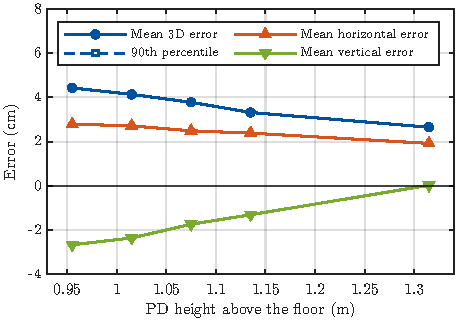
\includegraphics[width=\linewidth]{fig_grid_height.pdf}
 \caption{Error versus PD height on D2 (25 positions per height, $K=10$): mean and 90th percentile of the 3D error, mean horizontal error and mean signed vertical error.}
 \label{fig:height}
\end{figure}

\subsection{Number of Orientations}
\label{subsec:res-K}
Subsampling the ten angles of D2 shows how few orientations suffice (Fig.~\ref{fig:cdf}). The mean error is 3.66~cm with $K=10$, 3.74~cm with $K=5$ (P90 5.98~cm), 3.97~cm with $K=4$ and 4.95~cm with $K=3$ (P90 8.07~cm), and no estimate fails, not even with three orientations. Beyond $K=5$ the additional orientations do not reduce an error that is dominated by model bias; with $K=3$ the problem is exactly determined and no redundancy is left against these biases, which shows mainly in the tail of the distribution.

\begin{figure}[!t]
 \centering
 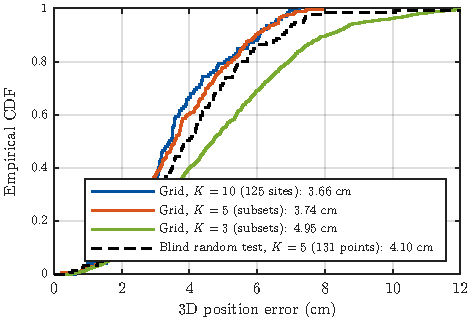
\includegraphics[width=\linewidth]{fig_cdf.pdf}
 \caption{Empirical CDF of the 3D error: D2 with $K=10$ and with near-uniform subsets of $K=5$ and $K=3$ angles, and the blind random test D3 ($K=5$). The legend gives the mean errors.}
 \label{fig:cdf}
\end{figure}

\subsection{Calibration Budget}
\label{subsec:res-budget}
Because the direction and amplitude of every position do not depend on $A$ and $m$, the error on D2 can be recomputed exactly for any calibration. Fig.~\ref{fig:calibration}(b) does so for calibrations obtained from $N$ points of D1 with the LED position known. A regular $n\times n$ grid over the working area reaches the accuracy of the full map with very few points: 3.45, 3.54 and 3.57~cm for $2\times2$, $3\times3$ and $4\times4$, against 3.65~cm with all 19\,881 points. Random points over the area need about ten to approach it (median 3.86~cm for $N=10$). Concentrating the points around the LED, which looks natural, fails: a $3\times3$ grid with 0.1 or 0.2~m spacing centered on the LED gives 21.8 and 17.3~cm, and it recovers only when the spacing reaches 0.4~m (4.16~cm). The reason is the angle-dependent apparent order of Fig.~\ref{fig:calibration}(a): points near the axis push $m$ upwards, and the calibration must sample the emission angles at which the system operates. No pair $(A,m)$ does better than 3.15~cm on D2, even when chosen with the ground truth; this is the floor of the single-order pattern model, reached within 0.5~cm by nine well-placed points.

\begin{figure}[!t]
 \centering
 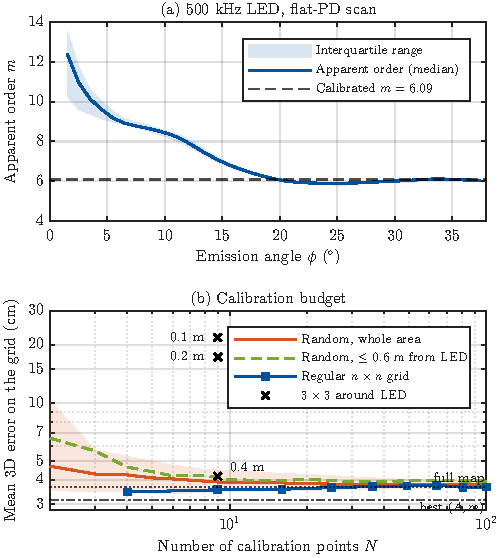
\includegraphics[width=\linewidth]{fig_calibration.pdf}
 \caption{LED calibration on D1 (500~kHz). (a)~Apparent Lambertian order versus emission angle, with $A$ fixed by the point closest to the axis. (b)~Mean 3D error on D2 when $A$ and $m$ come from $N$ points of D1: regular grids over the working area, random points over the area (median and P10--P90 over 400 draws) or within 0.6~m of the LED, and $3\times3$ grids centered on the LED with the indicated spacing. Horizontal lines: full-map calibration and best possible $(A,m)$.}
 \label{fig:calibration}
\end{figure}

\subsection{Blind Random Test}
\label{subsec:res-blind}
On the 131 random positions of D3, estimated live with $K=5$ and the calibration frozen beforehand, the mean 3D error is 4.10~cm (median 3.91~cm, RMSE 4.53~cm, P90 6.73~cm, maximum 12.5~cm), with a mean horizontal error of 2.64~cm, a mean vertical error of $-1.96$~cm and a mean direction error of $0.90^\circ$ (Figs.~\ref{fig:cdf} and~\ref{fig:random}). Recomputing these estimates offline from the stored RSS reproduces the live values within 0.002~cm. The result is close to the $K=5$ subsets of D2 (3.74~cm); the slightly larger error and tail come from positions near the edges of the area and near the lowest height, which the regular grid samples less densely, and from the stage zero, which in D3 is no longer refitted. The accuracy measured on the regular grid thus transfers to unseen positions.

\begin{figure*}[!t]
 \centering
 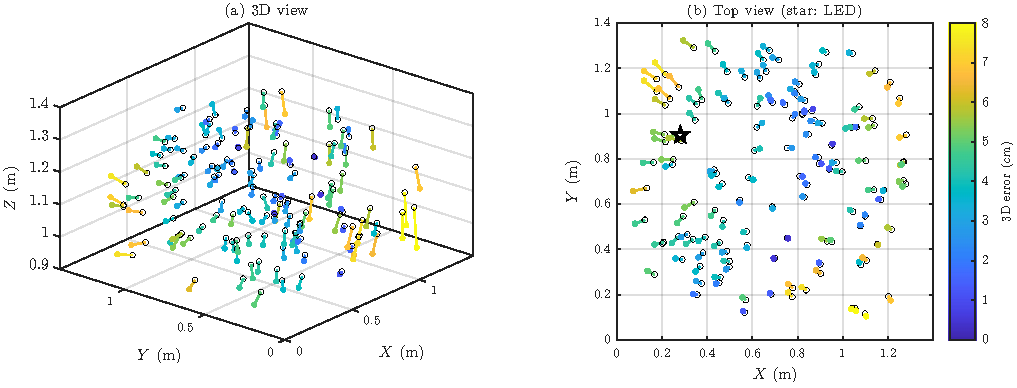
\includegraphics[width=\textwidth]{fig_random.pdf}
 \caption{Blind random test D3 (131 positions, $K=5$): true positions (hollow) and estimates (filled, colored by the 3D error), joined by their error vectors. (a)~3D view; (b)~top view, with the LED (star).}
 \label{fig:random}
\end{figure*}

\subsection{Integrity Monitoring}
\label{subsec:res-integrity}
During the first session of D3, the tilt axis of the stage moved by itself from the 48th position on, while it was not commanded; its encoder then reported up to $2.85^\circ$. Fig.~\ref{fig:integrity} shows the residual $\hat\rho$ of the fit at every position of that session. Its median rises from 0.42\,\% before the fault to 1.74\,\% after it, while the mean 3D error grows from 3.28 to 13.9~cm (maximum 25.1~cm). A threshold of 0.9\,\%, the largest residual observed on the fault-free grid D2, is exceeded by 82\,\% of the faulty positions but also by 11.5\,\% of the valid positions of D3, because five orientations give noisier residuals than ten. Requiring two consecutive exceedances removes all false alarms over the 131 valid positions and raises the alarm at the 51st position, four positions after the onset (three consecutive exceedances: 52nd). The residual therefore detects that the assumed orientations are wrong without any ground truth, which is why these 44 positions are excluded from D3. A later dense-grid campaign, in which the rotation stage slipped while its encoder kept reporting the commanded angles, was discarded for the same reason.

\begin{figure}[!t]
 \centering
 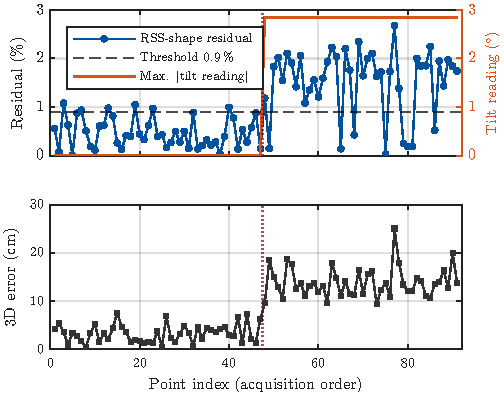
\includegraphics[width=\linewidth]{fig_integrity.pdf}
 \caption{Session affected by a fault of the stage (tilt axis moving by itself from position 48, dotted line). Top: residual $\hat\rho$ of the fit and maximum tilt reported by the stage encoder; dashed line: threshold. Bottom: 3D error.}
 \label{fig:integrity}
\end{figure}

\subsection{The Other LEDs as Single-LED Systems}
\label{subsec:res-leds}
The 300, 700 and 900~kHz LEDs are recorded in every measurement and provide three more single-LED systems with the same receiver and positions. Each was calibrated ``from scratch'' on D1 like the 500~kHz LED and used alone to position the 125 sites of D2 (Table~\ref{tab:leds}). Two LED positions are compared: the center of the pattern, fitted on D1 together with $A$ and $m$, and the geometric position, obtained by intersecting the directions to that LED estimated at the known positions of D2, which do not depend on its gain or pattern. To avoid evaluating on the data used to locate the LED, the geometric position used at each height is triangulated from the other four.

The calibration budget holds for every LED: $3\times3$ and $4\times4$ grids give the same accuracy as the full map. The accuracies, however, differ widely, from about 3~cm (500~kHz) to 17--24~cm (700~kHz), and the difference between the two LED positions reveals why. For the 700~kHz LED the pattern center lies 17.9~cm from the geometric position, which corresponds to a tilt of about $5.5^\circ$ of its optical axis over the 1.865~m between the LED and the scan plane; the other LEDs show tilts of $0.8^\circ$ to $1.9^\circ$. The model assumes a vertical axis, so a tilted LED biases the calibrated pattern, and no number of calibration points can compensate for it. Using the geometric position improves every LED, but only a model with the LED tilt, or a realigned LED, would remove the bias. The triangulated LED heights, 2.95--2.97~m, are 3--5~cm below the tape value, consistent with the small negative vertical errors of the estimates. Read in reverse, the method diagnoses the installation: it measures where each LED is and where it points, from the same data used for positioning.

\begin{table*}[!t]
 \centering
 \caption{Each LED Used Alone (D2, 125 Positions, $K=10$)}
 \label{tab:leds}
 \small
 \setlength{\tabcolsep}{8pt}
 \begin{tabular}{@{}lcccc@{}}
 \toprule
 LED & 300~kHz & 500~kHz & 700~kHz & 900~kHz\\
 \midrule
 Pattern center (mm) & (1177, 1175) & (284, 905) & (205, 508) & (1164, 235)\\
 Geometric position (mm) & (1205, 1176) & (306, 890) & (317, 368) & (1194, 181)\\
 Shift / tilt & 2.8~cm / $0.9^\circ$ & 2.6~cm / $0.8^\circ$ & 17.9~cm / $5.5^\circ$ & 6.2~cm / $1.9^\circ$\\
 \midrule
 \multicolumn{5}{@{}l}{Mean 3D error (cm), LED at the pattern center:}\\
 \quad $3\times3$ points & 7.08 & 3.48 & 24.49 & 12.96\\
 \quad all points & 8.61 & 3.42 & 23.67 & 13.44\\
 \multicolumn{5}{@{}l}{Mean 3D error (cm), LED at the geometric position:}\\
 \quad $3\times3$ points & 6.22 & 2.92 & 17.00 & 6.57\\
 \quad all points & 5.56 & 3.08 & 16.93 & 5.62\\
 \bottomrule
 \end{tabular}
\end{table*}

\subsection{Comparison With the Position Error Bound}
\label{subsec:res-bound}
Fig.~\ref{fig:peb}(a) compares the measured errors on D2 with the bound evaluated at the same positions and orientations. With the measured noise and exactly known normals, the median bound is 0.75~mm for $K=10$ (P90 1.61~mm) and 1.06~mm for $K=5$; including the relative fluctuation of consecutive records raises it to 0.94~mm. The median measured error is about 39 times larger: the system is far from noise-limited. The bound with orientation uncertainty indicates what this gap is made of. An uncertainty of only $0.1^\circ$ per tangent component already raises the median bound to 4.1~mm, $0.5^\circ$ to 2.0~cm and $1^\circ$ to 4.0~cm; the measured errors lie between the last two curves. Small angular errors in the model thus explain errors of a few centimeters, and the measurements show several such sources: the stage zero, fitted per height, drifts by about $0.5^\circ$ over the ten hours of D2; the estimated directions carry the small elevation bias revealed by the triangulated LED heights; and the single-order pattern model alone has a floor of 3.15~cm (Section~\ref{subsec:res-budget}), which~\eqref{eq:range-sensitivity} links to direction errors of the order of one degree. Further accuracy will come from better models of the LED and of the receiver orientation, not from more averaging, power or orientations.

\subsection{Acquisition Time}
\label{subsec:res-time}
A position of D2 ($K=10$) took 4.2~min on average, and a position of the live test ($K=5$) 3.7~min. About 87\,\% of this time is the rotation of the stage at $1.5^\circ$/s; each record, including its transfer, takes about one second. The duration is a property of the actuator, not of the method: a stage rotating at about $20^\circ$/s would bring a five-orientation position below one minute.
